\documentclass[a4paper]{article}
\usepackage{graphicx}
\usepackage[ngerman]{babel}
\usepackage[utf8]{inputenc}
\usepackage{color}
\usepackage{geometry}
\geometry{verbose,a4paper,tmargin=30mm,bmargin=25mm,lmargin=20mm,rmargin=20mm}

%opening
\author{Kira von Horsten, Doreen Schwarze}

\begin{document}
\thispagestyle{empty}
\begin{center}

\includegraphics[width=10cm]{Uni}
\section*{\textcolor{blue}{\textbf{Unsere Universität}}\\\textit{Our University }}
\vspace{1cm}
\begin{small}
\textbf{Bachelorarbeit}\\ 
\vspace{1cm }
im Rahmen des Studiengangs\\
\textbf{Medieninformatik}\\
der Universität zu Lübeck
\end{small}
\vspace{1.5cm}\\ vorgelegt von:\\ \textbf{Vorname Nachname des Studierenden}
\vspace{1.5cm}\\ ausgegeben und betreut von:\\ \textbf{Prof. Dr. Erika Musterfrau}
\vspace{1.5cm}\\ mit Unterstützung von:\\ \textbf{Lieschen Müller}\\

\vspace{1cm}Lübeck, 22.11.2016
\end{center}
\newpage 
\thispagestyle{empty}
\quad 
\newpage
\pagenumbering{Roman}
\setcounter{page}{3}
\vspace*{\fill}
\subsection*{Erklärung}
Hiermit erkläre ich, dass ich einen Wikipediaartikel übernommen habe. Daten und Konzepte sind unter Angabe des Literaturzitats gekennzeichnet.\\
\newline
\newline
\newline
\underline{\hspace{7 cm}}
\newline
(Name des Studenten)\\\Lübeck,den 22.11.2016

\newpage 
\thispagestyle{empty}
\quad 
\newpage
\pagenumbering{Roman}
\setcounter{page}{5}
\section*{Kurzfassung}
Die Universität zu Lübeck ist eine Hochschule in der Hansestadt Lübeck (Deutschland), die 1964 zunächst als zweite Medizinische Fakultät der Universität Kiel eingerichtet wurde. Studienangebot und Forschungstätigkeit der Universität zu Lübeck haben ihren Ausgangspunkt in der Medizin.\\
\noindent Die Universität zu Lübeck trägt diesen Namen seit Mai 2002. Sie wurde 1964 als Medizinische Akademie Lübeck gegründet. 1973 wurde sie selbstständige wissenschaftliche Hochschule, zunächst unter dem Namen Medizinische Hochschule Lübeck, seit 1985 als Medizinische Universität zu Lübeck.

\newpage 
\thispagestyle{empty}
\quad 
\newpage
\pagenumbering{Roman}
\setcounter{page}{7}
\section*{Abstract}
The University of Lübeck is a research university in Northern Germany which focuses almost entirely on medicine and sciences with applications in medicine. In both 2006 and 2009, the University of Lübeck was ranked No. 1 in medicine among all universities in Germany, Austria and Switzerland according to the CHE Hochschulranking. In Computer Science and Molecular Life Science, the University was ranked No. 2 in the 2009 evaluation.

\newpage 
\thispagestyle{empty}
\quad 
\newpage
\pagenumbering{Roman}
\setcounter{page}{9}

\tableofcontents
\newpage

\newpage
\thispagestyle{empty}
\quad 
\newpage
\pagenumbering{arabic}     
\setcounter{page}{1}
\section{Einleitung}
An der Universität sind etwa 3.900 Studenten, 160 Professoren und 100 Privatdozenten tätig. Das Universitätsklinikum Lübeck wurde am 1. Januar 2003 mit dem Universitätsklinikum Kiel zum Universitätsklinikum Schleswig-Holstein und damit zum zweitgrößten Universitätsklinikum Deutschlands zusammengeschlossen. Mit über 5300 Mitarbeitern gehören die Universität und das Klinikum zu den größten Arbeitgebern der Region Lübeck.\\

\noindent Zurzeit bestehen 14 Institute in der Sektion Informatik/Technik, darunter Grundlagenfächer wie Mathematik und Theoretische Informatik und neue Disziplinen wie Telematik oder das Institut für Multimediale und Interaktive Systeme; weitere acht Institute in der Sektion Naturwissenschaften, hierbei auch das geisteswissenschaftliche Institut für Medizingeschichte und Wissenschaftsforschung. Die Sektion Medizin beinhaltet 39 Institute. Im Lübecker universitären Bachelor- und Master-Studiengang Informatik stehen die Nebenfächer Medizinische Informatik, Bioinformatik/Biomathematik, Robotik und Automation, Medieninformatik sowie IT-Sicherheit und Zuverlässigkeit, sowie nur für Masterstudenten Software Systems Engineering, zur Auswahl.[3]\\

\noindent Neben den Vollstudiengängen führt die Universität gemeinsam mit der Fachhochschule Lübeck den Master-Studiengang „Biomedical Engineering“ durch. An der Universität besteht in Kooperation mit der Fernuniversität Hagen ein Zentrum für Fernstudium und Weiterbildung. Das Studium Generale und die Sonntagsvorlesungen wenden sich auch an Nicht-Studenten. Das auf Anregung von Günter Grass und mit seiner Unterstützung gegründete Lübecker Literarische Colloquium bietet regelmäßige Dichterlesungen und Seminare über Literatur an.\\

\noindent Wissenschaftlich ist die Universität eng mit dem Forschungszentrum Borstel (Zentrum für Medizin und Biowissenschaften) und dem Institut für Krebsepidemiologie (Registerstelle des Krebsregisters Schleswig-Holstein) verbunden.\\

\noindent Die Universität war an den Planungen der Hansestadt Lübeck und des Landes Schleswig-Holstein zum Hochschulstadtteil Lübeck auf dem Gelände des ehemaligen Gutes Strecknitz beteiligt. Das stadtplanerische Konzept mit Modellcharakter umfasst insbesondere den Aufbau eines Wissenschafts- und Technologieparks (WTP) „Innovations-Campus Lübeck“ für einen intensiven Transfer zwischen Universität und Firmenneugründungen.\\

\noindent Außerdem ist die Universität am Verbund Norddeutscher Universitäten zur Verbesserung von Lehre und Forschung beteiligt.
\newpage
\section{Geschichte}
Im Jahr 1912 wurde die Heil- und Pflegeanstalt Strecknitz eröffnet, Grundsteinlegung war 1909. In der Zeit des Nationalsozialismus wurden im Zuge der „Aktion Brand“ aus der Heilanstalt 605 der psychiatrischen Patienten nach Eichberg in Hessen deportiert. Dies wurde erst 1983 durch einen Gedenkstein auf dem Klinikgelände öffentlich gemacht. Der Gedenkstein wurde aufgestellt, nachdem eine 1981 vom AStA der Universität in Zusammenarbeit mit dem Institut für Medizingeschichte organisierte Ringvorlesung zum Thema „Medizin und Nationalsozialismus“ auf das Schicksal der Patienten aufmerksam gemacht hatte. Nach 1945 war die Einrichtung das Städtische Krankenhaus Ost.\\

\noindent Am 3. November 1964 entstand aus dem Campus die Medizinische Akademie Lübeck (II. Medizinische Fakultät der Christian-Albrechts-Universität Kiel), an der im ersten Jahr 14 Studenten ihr Studium im klinischen Abschnitt des Studiengangs Humanmedizin aufnehmen. Das Siegel, das Lübsche Stadtsiegel von 1226, wurde der Akademie 1965 von der Stadt Lübeck verliehen. Es ist bis heute in abgewandelter Form das Siegel der Universität. Der Lehrbetrieb wurde in dieser Zeit noch zwischen Krankenhaus Ost und Süd aufgeteilt. Da einige Lehrstühle unbesetzt waren, mussten Studenten für manche Examen nach Kiel fahren.[10] Am 7. Mai 1973 wurde die Akademie in Medizinische Hochschule Lübeck umbenannt und somit unabhängig von der Universität Kiel.\\

\noindent 1979 kam die Vorklinisch-Naturwissenschaftliche Fakultät hinzu (heute: Sektion MINT), der Studienbetrieb im vorklinischen Abschnitt des Medizinstudiums wurde aufgenommen. Am 10. Mai 1985 erfolgte die Umbenennung in Medizinische Universität zu Lübeck. Im Wintersemester 1993/1994 wurde der neue Studiengang „Informatik“ mit dem Nebenfach „Medizinische Informatik“ aufgenommen, in den Folgejahren werden andere Vertiefungen etabliert. Seit dem Wintersemester 2001/2002 können Studenten sich für den Studiengang „Molekulare Biotechnologie“ (seit Sommersemester 2004: „Molecular Life Science“) einschreiben. Am 29. Mai 2002 erfolgte die Umbenennung in „Universität zu Lübeck“. Im Wintersemester 2002/2003 kam der Studiengang „Computational Life Science“ (seit 2010: „Angewandte Mathematik in Naturwissenschaften und Medizin“) hinzu.\\

\noindent Nach Plänen der Landesregierung, im Herbst 2005 die Universitäten Kiel und Lübeck zur Landesuniversität Schleswig-Holstein zusammenzulegen, kam es in Lübeck zu Protesten. Über 4000 Lübecker gingen auf die Straße und protestierten, die Pläne konnten abgewandt werden.\\

\noindent Am 1. November 2007 wurde die Graduate School „Computing in Medicine and Life Sciences“ im Rahmen der Exzellenzinitiative des Bundes und der Länder eingerichtet. Seit dem Wintersemester 2007/2008 gibt es den neuen Studiengang „Medizinische Ingenieurwissenschaft“.
Plakat vom AStA der Uni Lübeck
Einer der Züge des Sternmarsches vom 1. Juli 2010
Protestbanner am Holstentor\\

\noindent Die Kieler Landesregierung plante im Mai 2010, aus Kostengründen die medizinische Fakultät zu schließen.[11] Geplant war ein Auslaufen der Studiengänge ab Wintersemester 2011/2012 und eine Verlagerung an die Universität Kiel.[12] Folge war eine Abwanderung der Professoren, vor allem aus der Forschung.[13] Die Schließung des Medizinstudienganges stieß in den Folgemonaten auf heftige Kritik in der Öffentlichkeit,[14] in der Wissenschaft,[15] in der Politik[16] und sogar innerhalb der CDU.[17] Es erfolgte eine weitgehend vom AStA der Universität organisierte Protestaktion Lübeck kämpft mit zahlreichen Mitstreitern im Lübecker Raum.[18] Am 16. Juni 2010 demonstrierten in Kiel 14.000 Menschen gegen die Schließung der medizinischen Fakultät, es war die größte Demonstration in Kiel in der Geschichte Schleswig-Holsteins.[19][20] Am 8. Juli 2010 konnte der Fortbestand der medizinischen Ausbildung in Lübeck dadurch gesichert werden, dass der Bund finanzielle Zuwendungen im Rahmen eines Trägerwechsels des Kieler Instituts für Meeresforschung in Höhe der bei Schließung der medizinischen Fakultät Lübeck zu erwartenden Ersparnisse zusagte. Diese Zuwendungen sind an die Bedingung geknüpft, dass die medizinische Fakultät Lübeck erhalten bleibt.[21] Mehrere Stellen, hierunter die Universitätsleitung, regten wiederholt eine Umwandlung der Universität zu Lübeck in eine Stiftungsuniversität an, um künftig unabhängiger vom Land Schleswig-Holstein zu werden.\\
\newpage
\noindent Die Aktion „Lübeck kämpft“\cite{de_la_torre_approach} wurde im November 2010 mit dem von der Zeitschrift Politik und Kommunikation seit 2003 ausgelobten Preis „Politik-Award“ in der Kategorie „Kampagnen von öffentlichen Institutionen“ ausgezeichnet.[22]\\
\begin{figure}
\centerline{
\includegraphics[width=5cm]{kampf}}
\caption{Plakat vom AStA der Uni Lübeck}
\end{figure}\\

\noindent Zum Wintersemester 2013/2014 wird erstmals \cite{DBLP:conf/isola/Leucker0T16} für jeweils 40 Bachelor- und Master-Studenten der Studiengang Psychologie angeboten. Durch die Nähe zum Universitätsklinikum Schleswig-Holstein\cite{mueller2000}, Campus Lübeck (UK-SH) wird ein besonderer Schwerpunkt die Klinische Psychologie sein.\\

\noindent Seit 2015 ist die Universität zu Lübeck eine Stiftungsuniversität.

\begin{figure}[h]
\centerline{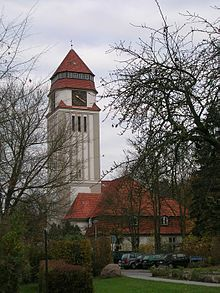
\includegraphics[width=5cm]{turm}}
\caption{Turmgebäude der Uni Lübeck}
\end{figure}
\begin{figure}[h]
\end{figure}

\newpage
\section{Institute}
Der Campus der Universität liegt südlich des Zentrums der Stadt im Stadtteil St. Jürgen. Einige Institute liegen außerhalb des Campus in der Lübecker Altstadt. Das Institut für Medizingeschichte und Wissenschaftsforschung verfügt als Leihgabe über die angesehene Bibliothek des Ärztlichen Vereins zu Lübeck.

\newpage
\section{Zusammenfassung und Ausblick}
Das Fazit aus der vorausgegangenen Arbeit ist, dass in der Stadt Lübeck eine sehr tolle Uni existiert. Diese wird wohl auch in Zukunft von vielen Studenten besucht werden.
\newpage
\bibliographystyle{alphadin}
\bibliography{literatur}

\end{document}
